\chapter{Феноменология нарушения CP-симметрии}\label{sec:phenom}
В этой главе рассмотрены основные феноменологические подходы к изучению нарушения \cpconj-симметрии в ускорительных экспериментах и описан экспериментальный статус изучения нарушения \cpconj-симметрии.% в распадах $B$-мезонов.

\section{Дискретные симметрии в Стандартной Модели}\label{sec:symmetries}
Симметрии играют фундаментальную роль в физической картине мира.  Соображения симметрии позволяют развивать теории на основе самых общих принципов.  Физический закон называют инвариантным (симметричным) относительно некоторого преобразования, если под действием этого преобразования \emph{вид} закона не меняется.  Так, все известные законы инвариантны относительно произвольного сдвига в пространстве: $\mathbf{r}\to \mathbf{r} + \delta \mathbf{r}$.  Преобразования и соответствующие им симметрии могут быть \emph{непрерывными} (например, произвольный сдвиг в пространстве) или \emph{дискретными} (например, пространственное отражение).

Согласно теореме Нётер~\cite{Noether1918}, каждой непрерывной симметрии соответствует некоторый закон сохранения.  Например, с однородностью и изотропностью пространства связаны соответственно законы сохранения импульса и момента импульса.

В теории квантовых полей важную роль играют дискретные преобразования и связанные с ними симметрии.  В частности, если теория соблюдает принципы локальности, релятивистской инвариантности и причинности, то лагранжиан такой теории будет инвариантен относительно \cptconj-преобразования, где \cconj означает оператор зарядового сопряжения, \pconj означает оператор пространственной четности, меняющий знак пространственных координат $\mathbf{r}\to-\mathbf{r}$, а \tconj означает оператор обращения времени $t\to-t$.   Калибровочные теории, являющиеся частью Стандартной Модели (СМ) элементарных частиц, построены согласно принципу \cptconj-инвариантности.

Наблюдения показывают, что электромагнитное и сильное взаимодействия инвариантны относительно \pconj- и \cpconj-преобразований, а слабое взаимодействие нарушает эти симметрии.  Нарушение \pconj-симметрии было экспериментально обнаружено в $1957$ году при изучении $\beta$-распада поляризованных ядер кобальта ${}^{60}Co$~\cite{Wu}.  Несохранение \pconj-четности связано со структурой лагранжиана слабого взаимодействия, в который входят векторные и псевдовекторные токи.  Первые меняют знак при \pconj преобразовании, в то время как вторые не меняются.

После обнаружения несохранения \pconj-четности Ландау выдвинул гипотезу о сохранении комбинированной \cpconj-четности в слабых взаимодействиях.  В $1963$ году, однако, несохранение \cpconj-четности (\cpconj-нарушение) в слабых взаимодействиях было обнаружено экспериментально при изучении распадов $K_L^0$-мезонов~\cite{CroninFitch}.  Кроме того, Сахаров отметил, что \cpconj-нарушение является одним из необходимых условий формирования барионной асимметрии~\cite{sakharov}.  
После этого Кобаяши и Маскава предложили механизм (\km-механизм), который в случае трех поколений кварков приводит к нарушению \cpconj-симметрии в слабых заряженных токов~\cite{km}.  Согласно \km-механизму, \cpconj-нарушающие эффекты во всей полноте проявляются в распадах $B$-мезонов, в которых задействованы кварки трех поколений.  Начавшие в $2003$ работу эксперименты \babar~\cite{BaBarNIM} и \belle~\cite{BelleNIM} на $B$-фабриках \pepii~\cite{PEPIICDR} (США) и \kekb~\cite{KEKB1} (Япония), соответственно, позволили детально изучить многие \cpconj-нарушающие феномены в распадах $B$-мезонов и подтвердить справедливость \km-механизма.

%\clearpage
\section{Механизм Кобаяши-Маскавы}\label{sec:ckm}
При описании процессов, обусловленных слабыми заряженными токами, полезной оказывается идея \emph{смешивания} кварковых полей.  Согласно этой идее, лагранжиан слабых заряженных токов описывает взаимодействие кварковых полей $q_u$ и $q_b^{\prime}$, где $q_u=\{u, c, t\}$ --- вектор полей верхних кварков, а $q_b^{\prime} = \{d^{\prime}, s^{\prime}, b^{\prime}\}$ --- вектор линейных комбинаций полей нижних кварков:
\begin{equation}\label{eq:ckm}
 \left(
 \begin{array}{c}
   d^{\prime} \\
   s^{\prime} \\
   b^{\prime} \\
  \end{array}
  \right)
  = \vckm
  \left(
  \begin{array}{c}
   d \\ s \\ b \\
  \end{array}
  \right)
  =
  \left(
  \begin{array}{ccc}
   V_{ud} & V_{us} & V_{ub} \\
   V_{cd} & V_{cs} & V_{cb} \\
   V_{td} & V_{ts} & V_{tb} \\
  \end{array}
  \right)\left(
  \begin{array}{c}
   d \\ s \\ b \\
  \end{array}
  \right),
\end{equation}
где $\vckm$ --- унитарная матрица смешивания кварков, называемая матрицей Кабиббо-Кобаяши-Маскавы (\ckm).  Матрица смешивания анти-кварков получается из матрицы \vckm с помощью комплексного сопряжения.  Таким образом, взаимодействие кварков отличается от взаимодействия анти-кварков, если $\vckm^*\neq \vckm$.  В общем виде матрица \vckm может быть параметризована с помощью четырех параметров: трех углов Эйлера ($\theta_{12}$, $\theta_{13}$ и $\theta_{23}$) и одной фазы~$\delta$~\cite{CKMEulerParams}:
\begin{equation}
 \vckm = 
 \lbr
 \begin{array}{ccc}
  c_{12}c_{13}                               &  s_{12}c_{13}                               & s_{13}e^{-i\delta} \\
 -s_{12}c_{23}-c_{12}s_{23}s_{13}e^{i\delta} &  c_{12}c_{23}-s_{12}s_{23}s_{13}e^{i\delta} & s_{23}c_{13}       \\
  s_{12}s_{23}-c_{12}c_{23}s_{13}e^{i\delta} & -c_{12}s_{23}-s_{12}c_{23}s_{13}e^{i\delta} & c_{23}c_{13}       \\
 \end{array}
 \rbr,
\end{equation}
где $c_{ij} = \cos{\theta_{ij}}$ и $s_{ij} = \sin{\theta_{ij}}$.  Фаза $\delta$ является единственным параметром \cm, отвечающим за нарушение \cpconj-симметрии.

На практике чаще применяется параметризация матрицы \ckm, предложенная Вольфенштейном~\cite{Wolfenstein}.  В этой параметризации \ckm-матрица записана в виде разложения по малому параметру~$\lambda$:
\begin{equation}\label{eq:wolf}
 \vckm = 
  \left(
  \begin{array}{ccc}
  1-\frac{\lambda^2}{2}               & \lambda               & A\lambda^3\left(\bar\rho-i\bar\eta\right) \\
  -\lambda                            & 1-\frac{\lambda^2}{2} & A\lambda^2                        \\
  A\lambda^3\left(1-\bar\rho-i\bar\eta\right) & -A\lambda^2           & 1 \\
  \end{array}
  \right)
  +\mathcal{O}(\lambda^4).
 \end{equation}
Экспериментальные значения параметров Вольфенштейна --- следующие~\cite{pdg}:
\begin{equation}\label{eq:wolf_param_values}
\begin{split}
 &\lambda = 0.22537\pm0.00061,\quad A = 0.814^{+0.023}_{-0.024},\\
 &\bar\rho = 0.117\pm0.021,\quad \bar\eta = 0.353\pm0.013.
\end{split}
\end{equation}

В случае двух поколений кварков, при подходящем выборе ненаблюдаемых комплексных фаз, матрица смешивания кварков может быть сведена к действительной матрице.  Такая матрица является двумерной матрицей поворота на угол \cabang, называемый углом Кабиббо~\cite{Cabibbo}.  Из уравнения \eqref{eq:wolf} видно, что параметр $\lambda$ соответствует величине $\sin\cabang$.  Именно существование трех поколений кварков естественно приводит к нарушению \cpconj-симметрии, хотя величина этого нарушения и не предсказывается.

Экспериментальная проверка описанного механизма нарушения \cpconj-симметрии сводится к измерению величин элементов \ckm-матрицы и проверке условия унитарности.  Наиболее подходящим для экспериментальной проверки является соотношение
\begin{equation}\label{eq:ut}
 \frac{V_{ud}V_{ub}^*}{V_{cd}V_{cb}^*}+\frac{V_{td}V_{tb}^*}{V_{cd}V_{cb}^*} + 1 = 0.
\end{equation}
Соотношение~\eqref{eq:ut} может быть представлено в виде треугольника на комплексной плоскости (рисунок~\ref{fig:UT}), называемого Треугольником Унитарности (\ut).  Вершины \ut находятся в точках $(0,0)$, $(1,0)$ и $(\bar\rho,\bar\eta)$, а величины углов выражаются через элементы \ckm-матрицы следующим образом:
\begin{equation}\label{eq:ut_angles}
 \aphi = \arg\lbr-\frac{V_{td}V^*_{tb}}{V_{ud}V^*_{ub}}\rbr,\quad
 \pphi = \arg\lbr-\frac{V_{cd}V^*_{cb}}{V_{td}V^*_{tb}}\rbr,\quad
 \gphi = \arg\lbr-\frac{V_{ud}V^*_{ub}}{V_{cd}V^*_{cb}}\rbr
\end{equation}
(в литературе также встречается альтернативное обозначение: $\aphi\equiv\varphi_2$, $\pphi\equiv\varphi_1$ и $\gphi\equiv\varphi_3$).  Измерение длин сторон и величин углов Треугольника Унитарности является одной из главных задач физики тяжелых кварков.

\begin{figure}[H]
 \centering
  \includegraphics[width=0.5\textwidth]{UT}
   \caption{Соотношение~\eqref{eq:ut}, представленное в виде треугольника на комплексной плоскости (Треугольник Унитарности)}
  \label{fig:UT}
\end{figure}

\section{Осцилляции нейтральных мезонов} \label{sec:mixing}
Четыре нейтральных мезона
\begin{equation}
 K^0(s\overline{d}),\quad
 D^0(c\overline{u}),\quad
 \bn(\overline{b}d),\quad
 \bs(\overline{b}s)
\end{equation}
и их античастицы не являются истинно-нейтральными частицами, т.е. не переходят в себя при \cpconj-сопряжении.  Во втором порядке по слабому взаимодействию существуют процессы, переводящие каждый из этих мезонов в соответствующий антимезон (и обратно).  Это означает, что состояния с определенным кварковым составом (\emph{ароматом}) не являются собственными (\emph{массовыми}) состояниями лагранжиана слабых взаимодействий.  Состояния с определенным ароматом (\pz, \pzb) связаны с массовыми состояниями (\pa, \pb) линейным преобразованием
\begin{equation}\label{eq:basis_transformation}
 \left(\begin{array}{c}
 \pb \\
 \pa
 \end{array}\right) 
 =
 \left(\begin{array}{cc}
 p & \phantom{-}q \\
 p & -q
 \end{array}\right )
 \left(
 \begin{array}{c}
 \pz \\
 \pzb
 \end{array}\right ),
\end{equation}
где $P$ обозначает любой из рассматриваемых нейтральных мезонов, индекс $\rmh$~($\rml$) соответствует состоянию с большей (меньшей) массой, $p$ и $q$ --- комплексные коэффициенты, ограниченные нормировочным условием $\left|p\right|^2 +\left|q\right|^2 = 1$.  Временная эволюция массовых состояний задается следующими соотношениями:
\begin{equation}\label{eq:mass_eig}
 \pat = e^{-im_{\rmh}t-\frac{\Gamma_{\rmh}}{2}t}\pati,\quad 
 \pbt = e^{-im_{\rml}t-\frac{\Gamma_{\rml}}{2}t}\pbti,
\end{equation}
где $m_{\{\rmh,\rml\}}$ и $\Gamma_{\{\rmh,\rml\}}$ обозначают соответственно массу и ширину состояний.  Уравнения~\eqref{eq:basis_transformation} и \eqref{eq:mass_eig} позволяют получить временную эволюцию состояний с определенным ароматом:
\begin{equation}\label{eq:flavor_states_evolution}
 \left (\begin{array}{c}\pzt\\\pzbt\end{array}\right )=
 \left (\begin{array}{cc}\kapp & i\frac{q}{p}\sigm\\
 i\frac{p}{q}\sigm & \kapp \end{array}\right )
 \left (\begin{array}{c}\pzti\\\pzbti\end{array}\right ),
 \end{equation}
где
\begin{equation}\label{eq:kap_sig}
 \begin{split}
 &\kapp = \emg\cos{\left(\frac{\dm t}{2}-i\frac{\dg t}{4}\right)},\\
 &\sigm = \emg\sin{\left(\frac{\dm t}{2}-i\frac{\dg t}{4}\right)},
 \end{split}
\end{equation}
и
\begin{equation}
 \dm \equiv m_{\rmh} - m_{\rml},\quad 
   m \equiv \frac{1}{2}(m_{\rmh}+m_{\rml}),\quad
 \dg \equiv \Gamma_{\rmh} - \Gamma_{\rml},\quad
   \Gamma \equiv \frac{1}{2}(\Gamma_{\rmh}+\Gamma_{\rml}).
\end{equation}

Осцилляции нейтральных мезонов играют важную роль в феноменологии \cpconj-нарушения (смотрите пункт~\ref{sec:cpv-phenom}).

\paragraph{\boldmath Осцилляции $B$-мезонов. }
Большая масса $b$-кварка, входящего в $B$-мезоны, определяет то, что переходы $\bn\leftrightarrow\bnbar$ происходят преимущественно за счет процессов на малых расстояниях (рисунок~\ref{fig:box-mixing}), без образования промежуточных связанных состояний (например, $\bn\to D^+D^-\to\bnbar$).  

\begin{figure}[htb]
   \centering
    \begin{minipage}[b]{0.49\textwidth}
  \centering
  \includegraphics[width=0.8\textwidth]{bmixing-box}
  \subcaption{}
 \end{minipage}
 \begin{minipage}[b]{0.49\textwidth}
  \centering
  \includegraphics[width=0.8\textwidth]{bmixing-box2}
  \subcaption{}
 \end{minipage}
   \caption{Процессы, определяющие переходы $\bn\leftrightarrow\bnbar$. $q$ обозначает промежуточные верхние кварки $\{u, c, t\}$.}
 \label{fig:box-mixing}
\end{figure}

Экспериментальное наблюдение осцилляций $B$-мезонов впервые выполнено группой ARGUS в $1987$ году~\cite{argus-bmix}.  В дальнейшем, осцилляции $B$-мезонов были детально изучены группами ALEPH~\cite{dmd-aleph}, DELPHI~\cite{al.2003}, L3~\cite{Acciarrietal.1998}, OPAL~\cite{Abbiendi2000266}, CDF~\cite{PhysRevD.60.072003}, D0~\cite{PhysRevD.74.112002}, CLEO~\cite{PhysRevLett.62.2233}, \babar~\cite{PhysRevD.73.012004}, \belle~\cite{flvtag1} и \lhcb~\cite{Aaij2013318}.  

Ширины массовых состояний нейтральных $B$-мезонов близки\footnote{Для $B_s^0$-мезонов это приближение не выполняется.}~\cite{hfag}, поэтому для простоту изложения мы пренебрежем их отличием (сравните с уравнением~\eqref{eq:kap_sig}):
  \begin{equation}\label{eq:kap_sig_b}
 \kappb=e^{-im_Bt}e^{-\frac{\gamb t}{2}}\cos{\frac{\dmb t}{2}},\quad
 \sigmb=e^{-im_Bt}e^{-\frac{\gamb t}{2}}\sin{\frac{\dmb t}{2}}.
 \end{equation}

Разность масс \dmb и время жизни $\btau\equiv 1/\gamb$ нейтральных $B$-мезонов измерены с высокой точностью~\cite{hfag}:
\begin{equation}
 \dmb = 0.5065 \pm 0.0019\ \ps{}^{-1},\quad \btau = 1.520 \pm 0.004\ \ps.
\end{equation}
На рисунке~\ref{fig:bmixing} показаны графики функций $|\kappb|^2$ и $|\sigmb|^2$, соответствующие измеренным параметрам.

\begin{figure}[htb]
 \centering
  \begin{minipage}[b]{0.49\textwidth}
  \centering
  \includegraphics[width=0.8\textwidth]{bmixing2}
  \subcaption{}
  \label{fig:bmixing}
 \end{minipage}
 \begin{minipage}[b]{0.49\textwidth}
  \centering
  \includegraphics[width=0.8\textwidth]{dmixing2}
  \subcaption{}
  \label{fig:dmixing}
 \end{minipage}
   \caption{ Графики функций а) $|\kappb|^2$ (непрерывная синяя линия), $|\sigmb|^2$ (пунктирная красная линия)  (уравнение~\eqref{eq:kap_sig_b}) и б) $|\sigmd|^2$ (уравнение~\eqref{eq:kap_sig_d}), описывающих временную эволюцию $B$- и $D$-мезонов.}
 \label{fig:mixing}
\end{figure}
 
\paragraph{\boldmath Осцилляции $D$-мезонов. }
Временная эволюция нейтральных $D$-мезонов заметно отличается от временной эволюции $B$-мезонов.  Вклад процессов на малых расстояниях (рисунок~\ref{fig:dmixing-box}) в переходы \dtodbar подавлен в соответствии с механизмом Глэшоу-Илиопулоса-Майяни~\cite{gim}, поскольку эти процессы в основном определяются кварками первых двух поколений.  Основной вклад в переходы \dtodbar дают процессы с образованием промежуточных мезонных состояний (рисунок~\ref{fig:dmixing-resonance})~\cite{petrov_charm}, поэтому теоретический расчет параметров осцилляций $D$-мезонов неизбежно сталкивается с трудностями, обусловленными необходимостью учета взаимодействия адронов на больших расстояниях.

\begin{figure}[htb]
 \centering
 \begin{minipage}[b]{0.49\textwidth}
  \centering
  \includegraphics[width=0.8\textwidth]{dmixing-box}
  \subcaption{}
  \label{fig:dmixing-box}
 \end{minipage}
 \begin{minipage}[b]{0.49\textwidth}
  \centering
  \includegraphics[width=0.8\textwidth]{dmixing-resonance}
  \subcaption{}
  \label{fig:dmixing-resonance}
 \end{minipage}
 \caption{Процессы, дающие вклад в переходы \dtodbar.}
 \label{fig:charm-mixing}
\end{figure}

Для описания осцилляций нейтральных $D$-мезонов вводят \emph{параметры смешивания}:
\begin{equation}
 x_D \equiv \frac{\Delta m_D}{\Gamma_D},\quad
 y_D \equiv \frac{\Delta\Gamma_D}{2\Gamma_D}.
\end{equation}

Экспериментальное наблюдение осцилляций $D$-мезонов впервые выполнено в $2007$ году группами \babar~\cite{babar_charm_mixing_observation} и \belle~\cite{belle_charm_mixing_observation}.  Группа \babar выполнила анализ распадов $\dn\to K^+\pi^-$, в которых был измерен параметр $y_D^{\prime} = -x_D\sin\delta_{K\pi} + y_D\cos\delta_{K\pi}$, где $\delta_{K\pi}$ обозначает разность фаз между амплитудами распадов $\dn\to K^+\pi^-$ и $\dnbar\to K^+\pi^-$:
\begin{equation}
 y_D^{\prime} = \lbr 9.7\pm4.4 \pm 3.1 \rbr \times 10^{-3}.
\end{equation}
Группа \belle опубликовала измерение параметра $y_D^{\cpconj}$, который равен параметру $y_D$ в случае сохранения \cpconj-симметрии в осцилляциях $D$-мезонов:
\begin{equation}
  y_D^{\cpconj} = \lbr 13.1\pm3.2\pm2.5 \rbr \times 10^{-3}.
\end{equation}
Это измерение выполненного посредством сравнения эффективных времен жизни \dn-мезона при его распаде в \cpconj-собственные конечные состояния ($K^+K^-$ и $\pi^+\pi^-$) и в конечное состояние $K^-\pi^+$. % Эти наблюдения подтверждают подавленность переходов \dtodbar.  

Прямые измерения параметров смешивания выполнены посредством времязависимого анализа распадов \dstpdpip, \dnkpp:
\begin{equation}
\begin{aligned}
&\left. \begin{array}{rl}
 x_D = (+0.56 \pm 0.19^{+0.03}_{-0.09}{}^{+0.06}_{-0.09})\times 10^{-2}   \\
 y_D = (+0.30 \pm 0.15^{+0.04}_{-0.05}{}^{+0.03}_{-0.06})\times 10^{-2}
       \end{array} \right\} & \belle~\text{\cite{peng_mixing}}, \\ %, \\
&\left. \begin{array}{rl}
 x_D = (+0.16 \pm 0.23 \pm 0.12 \pm 0.08)\times 10^{-2}   \\
 y_D = (+0.57 \pm 0.20 \pm 0.13 \pm 0.07)\times 10^{-2}
       \end{array} \right\} & \babar~\text{\cite{babar_dkspp_mixing}}, \\
&\left. \begin{array}{rl}
 x_D = (-0.86 \pm 0.53 \pm 0.17)\times 10^{-2}   \\
 y_D = (+0.03 \pm 0.46 \pm 0.13)\times 10^{-2}
       \end{array} \right\} & \lhcb~\text{\cite{lhcb_dkspp_mixing}}. \\
\end{aligned}
\end{equation}
Комбинация всех доступных в настоящее время измерений времени жизни нейтральных $D$-мезонов дает~\cite{pdg}
\begin{equation}\label{eq:dlifetime}
 \tau_D = 0.4101 \pm 0.0015\ps.
\end{equation}

Учитывая малость параметров смешивания, эволюционные коэффициенты~\eqref{eq:kap_sig} можно разложить в ряд Тейлора:
\begin{equation}\label{eq:kap_sig_d}
 \begin{split}
 &\kappd = \emdgd\left[1+                         \oxdydtsq\right],\\
 &\sigmd = \emdgd\left[\frac{\gamdt}{2}(x_D-iy_D)+\oxdydtsq\right].
 \end{split}
\end{equation}
На рисунке~\ref{fig:dmixing} показана функция $|\sigmd|^2$, дающая представление о малости эффекта осцилляций в системе нейтральных $D$-мезонов.

%\clearpage
\section{CP-нарушение в распадах B-мезонов} \label{sec:cpv-phenom}
Под нарушением \cpconj-симметрии в распадах $B$-мезонов понимают отличие вероятности перехода $B\to f$ от вероятности \cpconj-сопряженного перехода $\bbar\to\fbar$, где $f$ обозначает конечное состояние, $B = \{\bn,\ B^+\}$, $\bbar = \{\bnbar,\ B^-\}$, $\cpconj\left(f\right) = \fbar$ и $\cpconj\left(B\right) = \bbar$.  Если конечное состояние $f$ имеет кинематические степени свободы (три или более частицы в конечном состоянии), то различие дифференциальных вероятностей при сохранении полной вероятности также следует считать нарушением \cpconj-симметрии.  

Обозначим комплексную фазу элемента \ckm-матрицы, входящего в матричный элемент перехода, через $\varphi$.  Эта фаза меняет знак при \cpconj-сопряжении и обычно называется \emph{слабой} фазой.  Компонента $\delta$ комплексной фазы матричного элемента, инвариантная относительно \cpconj-преобразования, во многих случаях определяемая сильным взаимодействием, называется \emph{сильной} фазой.

В рамках \km-механизма, \cpconj-нарушение в распадах $B$-мезонов может возникнуть только при наличии \emph{двух} или более слагаемых в амплитуде перехода с различными сильными и слабыми фазами.  Действительно, рассмотрим состоящую из двух слагаемых амплитуду
\begin{equation}\label{eq:cpv_amp_sum}
 \mca = |\mca_1|e^{i(\delta_1+\varphi_1)}+|\mca_2|e^{i(\delta_2+\varphi_2)},
\end{equation}
такую, что $r \equiv |\mca_2|/|\mca_1|<1$.  Вероятность перехода пропорциональна квадрату модуля амплитуды перехода:
\begin{equation}\label{eq:cpv_amp_sum_norm}
 \mcp \equiv |\mca|^2 = \mcp_1\left[1 + r^2 + 2r\cos\left(\Delta\delta + \Delta\varphi\right)\right],
\end{equation}
где $\mcp_i\equiv |A_i|^2$, $\Delta\delta \equiv \left(\delta_2-\delta_1\right)$ и $\Delta\varphi \equiv \varphi_2-\varphi_1$. Вероятность \cpconj-сопряженного процесса пропорциональна
\begin{equation}
 \mcpbar \equiv |\mca|^2 = \mcp_1\left[1 + r^2 + 2r\cos\left(\Delta\delta - \Delta\varphi\right)\right],
\end{equation}
Набором необходимых и достаточных условий для отличия $\mcp$ от $\mcpbar$ является:
\begin{equation}
 r\neq0,\quad 
 \Delta\delta\notin \{0, \pi\} \quad 
 \varphi_1\notin \{0, \pi\}.
\end{equation}

Введем \emph{\cpconj-асимметрию} --- параметр, характеризующий степень нарушения \cpconj-симметрии:
\begin{equation}\label{eq:acp}
 \mca_\cpconj = \frac{\mcpbar-\mcp}{\mcpbar+\mcp} = \frac{2r\sin{\Delta\delta}\sin{\Delta\varphi}}{1+r^2+2r\cos{\Delta\delta}\cos{\Delta\varphi}},\quad |\mca_\cpconj|\leq1.
\end{equation}

Для наблюдения нарушения \cpconj-симметрии необходима интерференция между двумя (или более) процессами, приводящими к одному и тому же конечному состоянию.  Рассмотрим два примера, иллюстрирующие этот вывод и широко используемые для измерения углов~\ut.

\paragraph{\boldmath Измерение угла \gphi в распадах \bdk.} Распад \bdnkm происходит посредством кваркового перехода $b\to c\overline{u}s$ (рисунок~\ref{fig:BDKa}),  распад \bdbkm\ --- посредством кваркового перехода $b\to\overline{c}us$ (рисунок~\ref{fig:BDKb}).  Если нейтральный $D$-мезон переходит в конечное состояние~$f_D$, доступное для $D$-мезонов обоих ароматов, то  амплитуда процесса $B^-\to f_DK^-$ запишется в виде суммы
\begin{equation}\label{eq:bkd-amp}
 \mca_{\bdkm} = \mca_{\bdnkm}\mca_{\dn\to f_D} + \mca_{\bdbkm}\mca_{\dnbar\to f_D},
\end{equation}
Квадрат модуля амплитуды~\eqref{eq:bkd-amp} можно представить в следующем виде:
\begin{equation}\label{eq:p_bdkm}
 \mcp_{\bdkm} \equiv |\mca_{\bdkm}|^2 = 
 \mcp_{\bdnkm}\left|\mca_{\dn\to f_D} + \rb e^{i\lbr \delb+\gphi \rbr}\mca_{\dnbar\to f_D}\right|^2,
\end{equation}
где
\begin{equation}\label{eq:rb_deltab}
  \rb \equiv \left|\frac{\mca_{\bdbkm}}{\mca_{\bdnkm}}\right|,\quad
  \delb+\gphi = \arg\left(\frac{\mca_{\bdbkm}}{\mca_{\bdnkm}}\right).
\end{equation}
Величина \delb определяется сильным взаимодействием, в то время как слабая фаза определяется элементами \ckm-матрицы, входящими в амплитуды процессов, представленных на рисунке~\ref{fig:BDK}, и равна углу \gphi~\ut.  Измерения показали, что величина параметра \rb близка к $0.1$~\cite{lhcb_gamma_binned_dalitz,belle_gamma_dalitz_model,babar_gamma_dalitz_model}.

\begin{figure}[htb]
 \begin{minipage}[b]{0.5\textwidth}
  \centering
  \includegraphics[width=0.8\textwidth]{BDKfavAr}
  \subcaption{}
  \label{fig:BDKa}
 \end{minipage}
 \begin{minipage}[b]{0.5\textwidth}
  \centering
  \includegraphics[width=0.8\textwidth]{BDKsupAr}
  \subcaption{}
  \label{fig:BDKb}
 \end{minipage}
  \caption{Процессы, приводящие к распадам а)~\bdnkm и б)~\bdbkm}
  \label{fig:BDK}
\end{figure}

Вероятность \cpconj-сопряженного распада $B^+\to\fbar_DK^+$ запишем в следующем виде:
\begin{equation}\label{eq:p_bdkp}
 \mcp_{\bdkp} = \mcp_{\bdnkm}\left|\mca_{\dnbar\to\fbar_D} + \rb e^{i\lbr \delb-\gphi\rbr}\mca_{\dn\to\fbar_D}\right|^2.
\end{equation}

В работах~\cite{glw1,glw2} было предложено использовать \cpconj-собственные конечные состояния $D$-мезонов, такие как $K^+K^-$, $\pi^+\pi^-$ и $K_S^0\pi^0$.  В этом случае \cpconj-асимметрия~\eqref{eq:acp} выражается следующим образом:
\begin{equation}\label{eq:acp_glw}
 \mca_\cpconj^{(\glw)} = \frac{2\eta_D\rb\sin\delb\sin\gphi}{1+\rb^2+2\eta_Dr_B\cos\delb\cos\gphi},
\end{equation}
где $\eta_D$ --- \cpconj-четность конечного состояния $D$-мезона.

При рассмотрении распада \dkpi \cpconj-асимметрия принимает вид~\cite{ads}
\begin{equation}\label{eq:acp_ads}
 \mca_\cpconj^{(\ads)} = \frac{2\rd\rb \sin\left(\delb+\deld\right)\sin\gphi}{\rd^2+\rb^2+2r_Dr_B\cos\left(\delb+\deld\right)\cos\gphi},
\end{equation}
где
\begin{equation}\label{eq:rd_deltad}
 \rd e^{i\deld} = \frac{\mca_{\dn\to f_D}}{\mca_{\dnbar\to f_D}}.
\end{equation}
Данный подход может быть использован и при рассмотрении многочастичных адронных конечных состояний $D$-мезона, таких как $K^-\pi^+\pi^0$ и $K^-2\pi^+\pi^-$.  Для этого выражение~\eqref{eq:acp_ads} следует незначительно модифицировать~\cite{ads_multibody}.

Рассмотренные выше подходы не позволяют измерить значение параметра~\gphi из-за неизвестных адронных параметров \rb, \delb, \rd и \deld.  Преодолеть это ограничение позволяет использование трехчастичного распада \dkpp~\cite{bondar,GGSZ}.  Кинематика распада \dkpp описывается двумя параметрами, в качестве которых удобно использовать квадраты инвариантных масс пар частиц конечного состояния (переменные Далица~\cite{dalitz})
\begin{equation}\label{eq:dalitz_variables}
 m_{\pm}^2\equiv m^2\left(\ks\pi^{\pm}\right).
\end{equation}
При описании фазового пространства через переменные Далица плотность вероятности распада пропорциональна только квадрату модуля амплитуды:
\begin{equation}
 d\Gamma_{\dkpp} = \frac{1}{(2\pi)^3}\frac{1}{32m_D^3}\left|\mca\dvar\right|^2d\mpsq d\mmsq,
\end{equation}
где $m_D$ --- масса \dn-мезона, $\mca\dvar$ --- амплитуда распада \dnkpp.  Распределение событий в пространстве параметров Далица называют \emph{распределением Далица}; визуализация этого распределения называется \emph{диаграммой Далица} (рисунок~\ref{fig:kspp_dalitz}).  Предполагая сохранение \cpconj-симметрии в распаде $D$-мезонов, амплитуду распада \dbkpp можно записать с помощью перестановки переменных Далица: $\adbar\dvar \equiv \ad\dvarinv$.

\begin{figure}[htb]
 \centering
  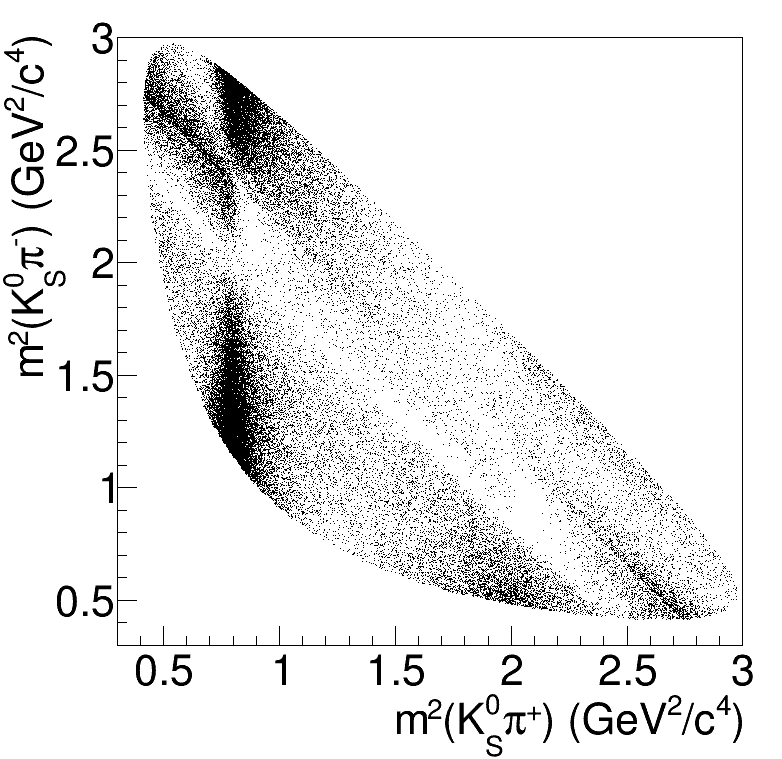
\includegraphics[width=0.45\textwidth]{dp_mc.png}
 \caption{Диаграмма Далица для распада \dbkpp.}
 \label{fig:kspp_dalitz}
\end{figure}

В случае распада \dkpp, параметры \rd и \deld (уравнение~\eqref{eq:rd_deltad}) являются функциями переменных Далица:
\begin{equation}
\begin{split}
 &\rd\dvar e^{i\deld\dvar} = \frac{\adbar\dvar}{\ad\dvar},\\
 & e^{i\deld\dvar} \equiv C\dvar + iS\dvar.
\end{split}
\end{equation}
Плотность распределения Далица для $D$-мезонов из распадов \bdk можно записать в виде
\begin{equation}\label{eq:dalitz_pdf_bdk}
\begin{split}
 \mcp_{B^+} &= \mcpdbar + \rb^2\mcpd    + 2\sqrt{\mcpd\mcpdbar}\left(x_+C + y_+S\right),\\
 \mcp_{B^-} &= \mcpd    + \rb^2\mcpdbar + 2\sqrt{\mcpd\mcpdbar}\left(x_-C - y_-S\right),
\end{split}
\end{equation}
где $\mcpd\equiv|\ad|^2$, $\mcpdbar\equiv|\adbar|^2$ и
\begin{equation}\label{eq:xy}
 x_{\pm} + iy_{\pm} \equiv \rb e^{i\left(\delb\pm\gphi\right)}.
\end{equation}
Зная функции \mcpd, $C$ и~$S$, можно измерить параметр~\gphi.  Обсуждение способов получения информации о функциях~$C$ и~$S$ приведено в пункте~\ref{sec:dalitz}.  

Чувствительность к параметрам~$x_{\pm}$ и~$y_{\pm}$ зависит от устройства функций $C$, $S$, \mcpd и~\mcpdbar (смотрите уравнение~\eqref{eq:dalitz_pdf_bdk}).  Для определения величины параметра~\gphi необходимо измерить все четыре параметра $x_{\pm}$ и $y_{\pm}$.  Необходимым условием для получения чувствительности ко всем этим параметрам является изменение разности фаз \deld (как функции переменных Далица) в широком диапазоне.  Наблюдения показывают, что распад \dnkpp обеспечивает достаточную чувствительность, а значительная вариация разности фаз~\deld достигается благодаря интерференции резонансных переходов $\dn\to\ks\rho$, $\dn\to\ks f_0$ и $\dn\to K^{*-}\pi^+$ (смотрите рисунок~\ref{fig:kspp_dalitz}).  

\paragraph{\boldmath Измерение угла \pphi с использованием осцилляций нейтральных $B$-мезонов.} Второй пример касается эффекта осцилляций нейтральных $B$-мезонов, рассмотренного в пункте~\ref{sec:mixing}.  Пусть в некоторое состояние $f_B$ могут распадаться нейтральные $B$-мезоны обоих ароматов.  Обозначим соответствующие амплитуды:
\begin{equation}
 \af \equiv \mca(\bn\to f_B),\quad \afbar \equiv \mca(\bnbar\to f_B).
\end{equation}
Если в начальный момент родился $B^0$-мезон, то амплитуда его перехода в состояние $f_B$ зависит от времени (в собственной системе отсчета) в соответствии с уравнением~\eqref{eq:flavor_states_evolution}:
\begin{equation}
 \ab(t) = e^{-imt-\Gamma t/2}\left[\af\cos\dmthalf + i\frac{q}{p}\afbar\sin\dmthalf\right].
\end{equation}
Соответствующая времязависимая плотность вероятности:
\begin{equation}\label{eq:time-dep-pb}
 \mcp_B(t) \propto e^{-\Gamma t}\left[1 + C_f\cos{\dmt} - S_f\sin{\dmt}\right],
\end{equation}
где 
\begin{equation}\label{eq:lamf}
 C_f = \frac{1-\lamfmsq}{1+\lamfmsq},\quad
 S_f = \frac{2\,\imag\,\lamf}{1+\lamfmsq},\quad
 \lamf=\frac{q}{p}\frac{\afbar}{\af}.
\end{equation}
\cpconj-асимметрия, определенная в~\eqref{eq:acp}, в рассматриваемом случае выражается через плотность вероятности~\eqref{eq:time-dep-pb} и является функцией времени~\cite{CarterSanda,BigiSanda}:
\begin{equation}\label{eq:time-dependent-acp}
 \acp\left(t\right) \equiv \frac{\mcpbar_B(t) - \mcp_B(t)}{\mcpbar_B(t) + \mcp_B(t)} = 
 S_f\sin{\dmt} - C_f\cos{\dmt}.
\end{equation}

При рассмотрении \cpconj-собственных конечных состояний $B$-мезонов и \cpconj-четностью $\eta_f$, амплитуда перехода в которые инвариантна относительно \cpconj-преобразования (например, $J/\psi\ks$), 
\begin{equation}\label{eq:qpbeta}
 \lamf = \eta_f e^{-2i\pphi},
\end{equation}
где угол \pphi определен в~\eqref{eq:ut_angles}, и асимметрия~\eqref{eq:time-dependent-acp} принимает вид
\begin{equation}\label{eq:time-dependent-acp-jpsi}
 \mca^{(J/\psi\ks)}_\cpconj\left(t\right) = -\sindbeta\sin{\dmt}.
\end{equation}

Описанный подход позволяет с высокой точностью измерить значение \sindbeta в распадах \bjpsiks.  Теоретическая неопределенность метода остается далеко за пределами чувствительности современных экспериментов.  В соответствии с общим принципом, чувствительность к \cpconj-нарушающему параметру обеспечена интерференцией двух процессов: $\bn\to f$ и $\bn\to\bnbar\to f$ (рисунок~\ref{fig:mixint}).

\begin{figure}[htb]
  \centering
  \includegraphics[width=0.4\textwidth]{mixing_interference}
  \caption{Схема интерференции процессов $\bn\to f$ и $\bn\to\bnbar\to f$.}
  \label{fig:mixint}
\end{figure}

Одной из проблем измерения параметра $2\pphi$ во времязависимом анализе \cpconj-собственных распадов $B$-мезонов является дискретная неопределенность $2\pphi\to\pi-2\pphi$.  Существует несколько способов разрешить эту неопределенность~\cite{Charles1998375,PhysRevD.56.7259,PhysRevD.61.116012}.  Наиболее привлекательный с экспериментальной точки зрения подход был рассмотрен в работе~\cite{bondar_gershon_krokovny}.  В этой работе предложено использовать распады \bdh, \dbkpp, где $h^0$ обозначает легкий нейтральный мезон (\pin, $\eta^{(\prime)}$ и $\omega$), и зависящую от времени в этом случае плотность распределения Далица для $D$-мезона из распадов \bdh:
\begin{equation}\label{eq:beta-dalitz-model-dep}
 \mcp_{q_B}\left(t\right) \propto e^{-\frac{t}{\btau}} \left[1 + q_B \left( \mca\dvar\cos{\dmt} + \mcs\dvar\sin{\dmt} \right)\right],
\end{equation}
где $q_B = 1$ ($q_B = -1$) соответствует \bn (\bnbar) при $t=0$ и
\begin{equation}
  \mca = \frac{\mcpd - \mcpdbar}{\mcpd + \mcpdbar},\quad
  \mcs = \frac{-2\eta_{h^0}(-1)^l\sqrt{\mcpd\mcpdbar}\sin{\left(\deld-2\pphi\right)}}{\mcpd + \mcpdbar},
\end{equation}
где $\eta_{h^0}$ --- \cpconj-четность $h^0$-мезона и $l$ --- орбитальный момент системы $Dh^0$.\footnote{Для распадов \bdstarh, \dbstdbpi, \dbkpp в функции \mcs возникает дополнительный множитель $-1$~\cite{bondar_gershon}.}  Значительное изменение разности фаз \deld в фазовом пространстве распада \dnkpp обеспечивает чувствительность к параметру $2\pphi$, значение которого может быть определено при известных функциях \mcpd, \mcpdbar и \deld.

% разработка алгоритма проверки и создание программ для измерения коэффициента усиления и линейности электронных модулей модернизированного калориметра Belle
% Bondar Gershon PRD 70, 091503(R)

\paragraph{\boldmath Классификация \cpconj-нарушающих распадов нейтральных $B$-мезонов.} \cpconj-нарушающие феномены в распадах нейтральных $B$-мезонов принято разделять на три группы:
\begin{enumerate}
 \item \emph{Прямое} нарушение \cpconj-симметрии. Реализуется при условии
 \begin{equation}
  \left|\frac{\afbar}{\af}\right|\neq 1.
 \end{equation}
 \item Нарушение \cpconj-симметрии \emph{в осцилляциях} нейтральных мезонов.  Реализуется при условии
 \begin{equation}
  \left|\frac{q}{p}\right|\neq 1.
 \end{equation}
 \item Нарушение \cpconj-симметрии \emph{в интерференции между осцилляциями и распадом}.  Реализуется при условии
 \begin{equation}
  \arg{\lamf}\neq 0.
 \end{equation}
\end{enumerate}
Приведенный пример нарушения \cpconj-симметрии в распадах \bjpsiks относится к \cpconj-нарушению в интерференции между осцилляциями и распадом.  %  В дальнейшем мы будем использовать эту терминологию.

%\clearpage
\section{Времязависимые измерения на асимметричной B-фабрике}\label{sec:dt_measurements}
Для изучения времязависимой \cpconj-асимметрии~\eqref{eq:time-dependent-acp} необходимо определять начальный аромат нейтрального $B$-мезона и измерять время между его рождением и распадом.  Эти требования приводят к большим экспериментальным сложностям, поскольку время жизни нейтральных $B$-мезонов примерно равно $1.5\ps$, а для определения аромата необходимо использовать информацию о частицах, рожденных вместе с $B$-мезоном.

Асимметричные ускорители встречных \ep-пучков высокой светимости, работающие вблизи резонанса~\ups ($B$-фабрики), были предложены для того, чтобы выполнение измерений такого рода было возможно.  Пара нейтральных $B$-мезонов, рожденных в процессе $\ep\to\ups\to\bn\bnbar$, находится в когерентном состоянии.  В соответствии с отрицательной \cconj-четностью \ups-резонанса, состояние пары $B$-мезонов антисимметрично относительно их перестановки.  Совместная плотность вероятности их распада во времена $t_1$ и $t_2$ (в собственных системах отсчета) может быть записана следующим образом~\cite{BaBarBook}:
\begin{equation}\label{eq:raw_coh_ampl}
 p(t_1,t_2) = p(\bn,t_1)p(\bnbar,t_2) - p(\bn,t_2)p(\bnbar,t_1),
\end{equation}
где $p(\bn, t_i)$ ($p(\bnbar, t_i)$) обозначает плотность вероятности того, что $B$ мезон, распавшийся в момент времени $t_i$, находится в состоянии с ароматом \bn (\bnbar). Плотности вероятности $p(\bn,t_i)$ и $p(\bnbar,t_i)$ определяются соотношением~\eqref{eq:flavor_states_evolution}.  

Пусть один из $B$-мезонов (\emph{помечающий}) распадается в состояние с определенным ароматом.  Тогда, благодаря антисимметричности состояния, в момент распада помечающего $B$-мезона, аромат второго (\emph{сигнального}) $B$-мезона определен и противоположен.

Рассмотрим плотность вероятности~\eqref{eq:raw_coh_ampl}, как функцию переменных $\dt\equiv (t_1 - t_2)$ и $(t_1+t_2)$. Проинтегрировав по переменной $(t_1+t_2)$, получим плотность вероятности распада сигнального $B$-мезона, как функцию переменной \dt
\begin{equation}\label{eq:time-dep-pb-tag}
 \mcp_B(\dt) \propto \bexp\left[1 + q_B\left(C_f\cos{\dmdt}-S_f\sin{\dmdt}\right)\right],
\end{equation}
где $q_B=1$ ($q_B=-1$) соответствует распаду сигнального $B$-мезона, как~\bn~(\bnbar).

Сумма масс двух $B$-мезонов близка к массе резонанса \ups, поэтому в системе \ups $B$-мезоны имеют небольшой импульс (примерно $300\mevc$) и характерный отлет около $30\mum$, измерить который с достаточной точностью не удается.  Для решения этой проблемы, энергии электронного и позитронного пучков делают разными, так что в лабораторной системе отсчета $B$-мезоны имеют достаточный для измерения отлета импульс и летят в направлении электронного пучка (в положительном направлении оси $z$, смотрите рисунок~\ref{fig:asym_collider}).  Используя малость импульса $B$-мезонов в системе отсчета \ups, можно получить кинематическое приближение
\begin{equation}\label{eq:kine-appr}
 \dt \approx \frac{\dz}{\cbgups},
\end{equation}
где \dz обозначает расстояние между вершинами распада $B$-мезонов в лабораторной системе отсчета, $\beta$ и $\gamma$ --- Лоренц-факторы резонанса \ups.  Таким образом, для получения разности времен распадов $B$-мезонов достаточно измерить координаты $z$ вершин их распадов.  Для $\bgups=0.425$ характерный отлет $B$-мезонов составляет примерно $200\mum$, поэтому для измерения координат вершин распадов необходим детектор с хорошей трековой системой, способной определять положение треков заряженных частиц с точностью лучше $100\mum$.

\begin{figure}[htb]
 \centering
  \includegraphics[width=0.7\textwidth]{collision_v2}
  \caption{Схема процесса $\ep\to\ups\to\bbbar$ на асимметричной $B$-фабрике.  \brec и \basc обозначают соответственно  сигнальный и помечающий $B$-мезоны.}
\label{fig:asym_collider}
\end{figure}

Анализ продуктов распада помечающего $B$-мезона позволяет получать информацию о его аромате (например, используя знак заряда лептона с большим импульсом или знак заряда $K$-мезона), необходимую для измерения \cpconj-асимметрии.  Таким образом, асимметричная $B$-фабрика позволяет выполнять измерения времязависимых \cpconj-асимметрий~\eqref{eq:time-dependent-acp}.

\section{Экспериментальный статус изучения CP-нарушения в распадах B-мезонов}\label{sec:angles}
В этом разделе представлен обзор основных экспериментальных результатов по изучению нарушения \cpconj-симметрии в распадах $B$-мезонов.

\subsection{CP-нарушение в древесных переходах}\label{sec:cpv_tree}
\paragraph{\boldmath Измерение \sindbeta в переходах \btoccs. } Кварковый процесс \btoccs происходит за счет древесного $b\to c$ перехода (рисунок~\ref{fig:btoccq_tree}) и петлевых $b\to s$ переходов (рисунок~\ref{fig:btoccq_loop}).  Амплитуду этого процесса можно представить в виде~\cite{bfacphys}
\begin{equation}\label{eq:amp_bccs}
 \mca_{\btoccs} = \vcb\vcsst\left(T + P^c - P^t\right) + \vub\vusst\left(P^u - P^t\right),
\end{equation}
где $T$ обозначает амплитуду древесного перехода, а $P^q$ --- амплитуду петлевого перехода с промежуточным кварком $q\in\{u, c, t\}$ (без соответствующих \ckm-множителей).  Вклад второго слагаемого со слабой фазой $V_{ub}$ в соотношении~\eqref{eq:amp_bccs} не приводит к значительным эффектам прямого \cpconj-нарушения, поскольку $|\vub\vusst/\vcb\vcsst|\sim\mco(\lambda^2)\sim 0.02$.  Доминирующая часть амплитуды~\eqref{eq:amp_bccs} пропорциональна $\vcb\vcsst$ и не содержит \cpconj-нарушающей фазы. 

\begin{figure}[htb]
\begin{minipage}[b]{0.5\textwidth}
 \centering
 \includegraphics[width=0.8\textwidth]{bccq_tree}
 \subcaption{}
 \label{fig:btoccq_tree}
\end{minipage}
\begin{minipage}[b]{0.5\textwidth}
 \centering
 \includegraphics[width=0.8\textwidth]{bccq_loop}
 \subcaption{}
 \label{fig:btoccq_loop}
\end{minipage}
 \caption{а) Древесный и б) петлевой вклады в переход \btoccq.}
 \label{fig:btoccq}
\end{figure}

Процесс \btoccs отвечает за распад $B^0$-мезона в \cpconj-собственное конечное состояние $\jpsi\ks$ с \cpconj-четностью $\eta_{\cpconj} = -1$ (мы пренебрегаем \cpconj-нарушением в системе нейтральных $K$-мезонов).  Благодаря тому, что \cpconj-нарушающая часть амплитуды распада \bjpsiks подавлена, этот распад позволяет изучать \cpconj-нарушение в интерференции между осцилляциями и распадом, как уже отмечалось.  При этом,
\begin{equation}\label{eq:acp_bccs}
 C_f(\bjpsiks) = 0,\quad S_f(\bjpsiks) = -\eta_\cpconj\sindbeta.
\end{equation}
Изучение времязависимой \cpconj-асимметрии в распадах \bjpsiks позволяет выполнять прецизионные измерения параметра \sindbeta (рисунок~\ref{fig:sindbeta_bccs}).  Самые точные на данный момент измерения выполнены в экспериментах \belle~\cite{belle_sinbeta}, \babar~\cite{babar_sinbeta} и \lhcb~\cite{lhcb_sinbeta}.  Комбинация всех существующих результатов измерений (включая использование конечных состояний $\jpsi K_L^0$, $\psiss\ks$, $\chi_{c1}\ks$ и некоторых других) дает~\cite{hfag} 
\begin{equation}\label{eq:sindbeta_bccs}
 \sindbeta^{(\btoccs)} = 0.691 \pm 0.017.
\end{equation}
Параметр \sindbeta является в настоящее время наиболее точно измеренным \cpconj-нарушающим параметром.

\begin{figure}[htb]
\begin{minipage}[b]{0.5\textwidth}
 \centering
 \includegraphics[width=\textwidth]{btoccsS_CP}
 \subcaption{}
 \label{fig:sindbeta_bccs}
\end{minipage}
\begin{minipage}[b]{0.5\textwidth}
 \centering
 \includegraphics[width=\textwidth]{phi1_rhoBar_etaBar}
 \subcaption{}
 \label{fig:beta_bccs}
\end{minipage}
 \caption{а) Результаты измерения \sindbeta в переходах \btoccs в различных экспериментах и б) ограничение на значение параметра \pphi, следующее из этих результатов~\cite{hfag}.}
 \label{fig:sinbeta}
\end{figure}

При известной величине \sindbeta, значение параметра \pphi может быть определено с точностью до двух дискретных неопределенностей
\begin{equation}
 \pphi \to \pi + \pphi,\quad \pphi \to \frac{\pi}{2} - \pphi.
\end{equation}
Первая из них не может быть разрешена любым измерением тригонометрических функций $2\pphi$, вторая же неопределенность может быть разрешена с помощью измерения параметра \cosdbeta.  При выборе области определения $\pphi\in[0\grad,180\grad)$, результат~\eqref{eq:sindbeta_bccs} соответствует решениям $(21.0\pm0.7)\grad$ и $(68.1\pm0.7)\grad$ (рисунок~\ref{fig:beta_bccs}).  

\paragraph{\boldmath Измерение \sindbeta в переходах \btocud. } Кварковый переход \btocud происходит благодаря единственной древесной амплитуде (рисунок~\ref{fig:btocudF}) и отвечает за распады нейтральных $B$-мезонов в такие конечные состояния, как $\dstarn h^0$ и $\dstarn\pi^+\pi^-$, где $h^0$ обозначает легкий мезон, состоящий из легких кварков: \pin, \etap и $\omega$.

\begin{figure}[htb]
\begin{minipage}[b]{0.5\textwidth}
 \centering
  \includegraphics[width=0.8\textwidth]{bcud}
 \subcaption{}
 \label{fig:btocudF}
\end{minipage}
\begin{minipage}[b]{0.5\textwidth}
 \centering
  \includegraphics[width=0.8\textwidth]{bucd}
 \subcaption{}
 \label{fig:btocudS}
\end{minipage}
 \caption{Кварковые переходы а) \btocud и б) \btoucd.}
 \label{fig:btocud}
\end{figure}

Рассматривая такие конечные состояния, как $D\pi^0$, где $D$-мезон распадается в \cpconj-собственное состояние, можно изучать времязависимую \cpconj-асимметрию и измерять \sindbeta аналогично случаю \btoccs переходов (смотрите уравнение~\eqref{eq:acp_bccs}).  Недавно группы \belle и \babar выполнили совместный анализ данных, используя набор из \cpconj-четных и \cpconj-нечетных конечных состояний, и получили следующее значение~\cite{markus_bdh}:
\begin{equation}\label{eq:sindbeta_bcud}
 \sindbeta^{(\btocud)} = 0.66 \pm 0.10\stat \pm 0.06\syst.
\end{equation}
Точность этого измерения значительно уступает точности измерения \sindbeta в переходах \btoccs~\eqref{eq:sindbeta_bccs}.  Тем не менее, этот результат важен с точки зрения ограничения возможных вкладов новой физики (НФ).  Кроме того, благодаря отсутствию петлевых вкладов, поправки к наблюдаемой величине нарушения \cpconj-симметрии в переходах \btocud меньше, чем соответствующие поправки в переходах \btoccs.  Основная поправка обусловлена кварковым переходом \btoucd (рисунок~\ref{fig:btocudS}), в результате которого происходят распады \bdnh.  Однако, амплитуда перехода \btoucd мала относительно амплитуды перехода \btocud, поскольку $|\vud\vcdst/\vcb\vudst|\approx 0.02$.  Кроме того, при достижении достаточной экспериментальной точности, вклад амплитуды \btoucd может быть учтен.

\paragraph{\boldmath Измерение \gphi в интерференции переходов \btocus и \btoucs.} В разделе~\ref{sec:cpv-phenom} обсуждалось прямое \cpconj-нарушение в распадах \bdk, возникающее благодаря интерференции процессов с переходами \btocus и \btoucs.  Изучение \cpconj-асимметрии в таких распадах позволяет получать информацию об угле \gphi~\ut.

Измерение \cpconj-асимметрии при реконструкции нейтральных $D$-мезонов в \cpconj-собственных конечных состояний (\glw-подход, уравнение~\eqref{eq:acp_glw}) выполнено с помощью анализа данных экспериментов CDF~\cite{cdf_glw}, \babar~\cite{babar_glw}, \belle и \lhcb~\cite{lhcb_glw_ads}.  Комбинация этих результатов дает значение
\begin{equation}
 \mca_{\cpconj+}^{(\glw)} =  0.125 \pm 0.017
\end{equation}
для конечных состояний с $\eta_\cpconj=1$ ($K^+K^-$, $\pi^+\pi^-$) и значение
\begin{equation}
 \mca_{\cpconj-}^{(\glw)} = -0.108 \pm 0.047
\end{equation}
для конечных состояний с $\eta_\cpconj=-1$ ($\ks\pin$, $\ks\omega$ и $\ks\varphi$).  На рисунке~\ref{fig:acp_glw} показаны результаты основных измерений $\mca_{\cpconj}^{(\glw)}$, включая результаты, полученные при анализе распадов $B^{\pm}\to D^{*}K^{\pm}$ и $B^{\pm}\to DK^{*\pm}$.

\begin{figure}[htb]
\begin{minipage}[b]{0.5\textwidth}
 \centering
  \includegraphics[width=0.99\textwidth]{A_cp}
 \subcaption{}
 \label{fig:acp_glw}
\end{minipage}
\begin{minipage}[b]{0.5\textwidth}
 \centering
  \includegraphics[width=0.99\textwidth]{A_ADS}
 \subcaption{}
 \label{fig:acp_ads}
\end{minipage}
 \caption{Результаты измерений а) $\mca_{\cpconj}^{(\glw)}$ (уравнение~\eqref{eq:acp_glw}) и б) $\mca_{\cpconj}^{(\ads)}$ (уравнение~\eqref{eq:acp_ads}) в распадах $B^{\pm} \to D^{(*)}_{\cpconj} K^{(*)\pm}$~\cite{hfag}.}
 \label{fig:acp_bdk}
\end{figure}

Измерение \cpconj-асимметрии при реконструкции нейтральных $D$-мезонов в состояниях с определенным ароматом (\ads-подход, уравнение~\eqref{eq:acp_ads}) выполнено в экспериментах CDF~\cite{cdf_ads}, \babar~\cite{babar_ads}, \belle~\cite{belle_ads} и \lhcb~\cite{lhcb_glw_ads}.  Наиболее точные результаты получены при реконструкции $D$-мезона в конечном состоянии $K^-\pi^+$.  Комбинация этих измерений дает
\begin{equation}
 \mca^{(\ads)}_{K\pi} = -0.41 \pm 0.06.
\end{equation}
На рисунке~\ref{fig:acp_ads} показаны результаты основных измерений $\mca^{(\ads)}$, включая результаты, полученные при реконструкции нейтральных $D$-мезонов в конечных состояниях $K^-\pi^+\pin$ и $K^-2\pi^+\pi^-$.

Использование распадов нейтральных $D$-мезонов в многочастичные \cpconj-самосопряженные состояния (например, \kspp, $\kspp\pin$ и $K^+K^-\pi^+\pi^-$) обеспечивает дополнительную чувствительность к параметру~\gphi~\cite{bondar,GGSZ}.  Конечное состояние \kspp позволяет проводить наиболее точные измерения, объединяя сильные стороны \glw- и \ads-подходов.  Основной вклад в распад \dnkpp вносят резонансы $\rho$, $f_0$ (приводя с \cpconj-собственном конечном состояниям $\ks\rho$ и $\ks f_0$) и $K^{*-}$ (приводя к конечному состоянию $K^{*-}\pi^+$ с определенным ароматом).  Интерференция этих резонансов увеличивает чувствительность к параметру \gphi и позволяет разрешить дискретные неопределенности, возникающие при извлечении величины этого параметра в \glw- и \ads-подходах.  

Как отмечалось ранее, для измерения \gphi в распадах \bdk, \dkpp необходимо иметь информацию об амплитуде распада $D$-мезона, включая разность фаз амплитуд распада \dn- и \dnbar-мезонов.  Распад \dnkpp представляет собой распад псевдоскалярной частицы в три псевдоскалярые частицы.  Это означает, что амплитуда распада является функцией в двумерном фазовом пространстве.  Информация об амплитуде может быть получена с помощью построения модели амплитуды трехчастичного распада, либо модельно-независимо.  В последнем случае фазовое пространство разделяется на области; для каждой области измеряется средние значения модуля амплитуды, синуса и косинуса комплексной фазы.  Подробнее эти вопросы обсуждаются в разделе~\ref{sec:dalitz}.

Результаты измерения \cpconj-нарушения в распадах \bdk, \dkpp принято выражать в декартовых параметрах $x_{\pm}$ и $y_{\pm}$ (уравнение~\eqref{eq:xy}).  Модельно-зависимые измерения этих параметров выполнены в экспериментах \babar~\cite{babar_gamma_dalitz_model}, \belle~\cite{belle_gamma_dalitz_model} и \lhcb~\cite{lhcb_gamma_dalitz_model} (рисунок~\ref{fig:bdk_unbinned_dalitz}).  Модельно-независимые измерения выполнены в экспериментах \belle~\cite{belle_gamma_binned_dalitz} и \lhcb~\cite{lhcb_gamma_binned_dalitz} (рисунок~\ref{fig:bdk_binned_dalitz}).

\begin{figure}[htb]
\begin{minipage}[b]{0.5\textwidth}
 \centering
  \includegraphics[width=0.99\textwidth]{D_DalitzKxvsy}
 \subcaption{}
 \label{fig:bdk_unbinned_dalitz}
\end{minipage}
\begin{minipage}[b]{0.5\textwidth}
 \centering
  \includegraphics[width=0.99\textwidth]{D_DalitzKmodIndxvsy}
 \subcaption{}
 \label{fig:bdk_binned_dalitz}
\end{minipage}
 \caption{Результаты измерений параметров $x_{\pm}$ и $y_{\pm}$, определенных в уравнении~\eqref{eq:xy}, в распадах \bdk, \dkpp с помощью а) модельно-зависимого и б) модельно-независимого анализа диаграмм Далица~\cite{hfag}.}
 \label{fig:bdk_dalitz}
\end{figure}

Группы \babar, \belle и \lhcb представили ограничения на величину параметра~\gphi, основываясь на комбинации всех полученных результатов:
\begin{equation}
 \begin{aligned}
  \gphi &= (69^{+17}_{-16})\grad     && (\babar~\text{\cite{babar_gamma}}), \\
  \gphi &= (68^{+15}_{-14})\grad     && (\belle~\text{\cite{belle_gamma}}), \\
  \gphi &= (70.9^{+7.1}_{-8.5})\grad && (\lhcb~\text{\cite{lhcb_gamma}}). \\
 \end{aligned}
\end{equation}
Комбинация этих результатов позволяет уменьшить неопределенность значения~\gphi приблизительно до~$6\grad$.

%\clearpage
% \subsection{CP-нарушение в петлевых переходах}\label{sec:cpv_loop}
% \begin{figure}[htb]
% \begin{minipage}[b]{0.32\textwidth}
%  \centering
%   \includegraphics[width=0.9\textwidth]{bsss}
%  \subcaption{}
%  \label{fig:bsss}
% \end{minipage}
% \begin{minipage}[b]{0.32\textwidth}
%  \centering
%   \includegraphics[width=0.9\textwidth]{bsll}
%  \subcaption{}
%  \label{fig:bsll}
% \end{minipage}
% \begin{minipage}[b]{0.32\textwidth}
%  \centering
%   \includegraphics[width=0.9\textwidth]{bsgamma}
%  \subcaption{}
%  \label{fig:bsgamma}
% \end{minipage}
%  \caption{Примеры петлевых переходов.}
%  \label{fig:loops}
% \end{figure}
% Распады, идущие в главном приближении посредством петлевых переходов, интересны с точки зрения проверки СМ, поскольку в петлях могут проявляться вклады НФ.  Примерами таких переходов являются радиационные и полулептонные переходы $b\to \{s,d\}\{\gamma,l^+l^-,\nu\overline{\nu}\}$, а также кварковые переходы \btosss, \btodds и \btossd (рисунок~\ref{fig:loops}).  
% 
% Интерпретация \cpconj-нарушающих феноменов в петлевых переходах осложняется тем, что необходимо учитывать вклады трех переходов с разными промежуточными кварками и разными слабыми фазами.  Эффекты адронизации также могут влиять на величину наблюдаемых \cpconj-нарушающих параметров.
% 
% \paragraph{\boldmath Поиск \cpconj-нарушения в адронных конечных состояниях. } Аналогично уравнению~\eqref{eq:amp_bccs}, амплитуду перехода \btosss можно представить в виде
% \begin{equation}\label{eq:amp_bsss}
%  \mca_{\btosss} = (P_c - P_u)\vcb\vcsst + (P_t - P_u)\vtb\vtsst.
% \end{equation}
% Относительная слабая фаза между двумя слагаемыми в уравнении~\eqref{eq:amp_bsss} мала и обозначается через
% \begin{equation}
%  \pphi_s\equiv\arg{\left(-\frac{\vts\vtbst}{\vcs\vcbst}\right)}.
% \end{equation}
% Поиск \cpconj-нарушения в распадах, обусловленных этим переходом ($B^+\to \varphi K^+$, $B^+\to\etap K^+$), является важным инструментом для проверки СМ.  Поиски \cpconj-нарушения в этих модах не выявили отклонений от СМ~\cite{babar_btokkk,lhcb_btokkk,belle_btoetapk,babar_btoetap}.  Комбинации измерений \cpconj-асимметрии (смотрите уравнение~\eqref{eq:acp}) согласуются с нулем: 
% \begin{equation}
%  \mca_\cpconj(B^+\to \varphi K^+) = 0.016\pm0.013,\quad \mca_\cpconj(B^+\to\etap K^+) = 0.004\pm0.011.
% \end{equation}
% 
% Относительная слабая фаза между петлевыми вкладами в переходе \btodds также равна $\pphi_s$, поэтому \cpconj-нарушающие эффекты в распадах $B^+\to \ks\pi^+$ ожидаются малыми, что согласуется с наблюдениями~\cite{belle_btohh,babar_btokk,lhcb_btokk}.
% 
% Б\emph{о}льшие \cpconj-нарушающие эффекты можно ожидать в переходах \btossd, поскольку относительная фаза петлевых амплитуд равна \pphi.  Распады, соответствующие этому кварковому переходу ($B^+\to \etap\pi^+$, $B^+\to\ks K^+$), однако, имеют небольшие вероятности, поэтому существующие наблюдения сильно ограничены статистически~\cite{lhcb_btokkk,belle_btoetapk,belle_btohh,babar_btokk,lhcb_btokk}.
% 
% \paragraph{\boldmath Измерение \sindbetaeff. } Переходы \btosss можно использовать для изучения времязависимой \cpconj-асимметрии (смотрите раздел~\ref{sec:cpv-phenom} и пункт~\ref{sec:cpv_tree}).  Параметр $S_f$ при этом выражают через \pphieff --- эффективный параметр \pphi:
% \begin{equation}
%  S_f^{(\btosss)} = -\eta_f\sindbetaeff.
% \end{equation}
% Величина \pphieff может отличаться от величины параметра \pphi, измеряемого в переходах \btoccs, из-за поправок, возникающих за счет петлевых вкладов.
% 
% \begin{figure}[htb]
% \begin{minipage}[b]{0.5\textwidth}
%  \centering
%   \includegraphics[width=0.99\textwidth]{sPengS_CP_woKsPi0Pi0}
%  \subcaption{}
%  \label{fig:bsssS}
% \end{minipage}
% \begin{minipage}[b]{0.5\textwidth}
%  \centering
%   \includegraphics[width=0.99\textwidth]{sPengC_CP_woKsPi0Pi0}
%  \subcaption{}
%  \label{fig:bsssC}
% \end{minipage}
%  \caption{Результаты измерения а) \sindbetaeff и б) коэффициента $C$ (смотрите уравнение~\eqref{eq:time-dependent-acp}) в кварковых переходах \btosss~\cite{hfag}.}
%  \label{fig:betaeff}
% \end{figure}
% 
% На рисунке~\ref{fig:bsssS} показаны результаты измерений параметра \sindbetaeff в распадах нейтральных $B$-мезонов, идущих  благодаря переходам \btosss.  На рисунке~\ref{fig:bsssC} приведены соответствующие результаты измерений коэффициента $C_f$, отвечающего за прямое нарушение \cpconj-симметрии.  Точность всех этих результатов ограничена статистической неопределенностью; наиболее точные измерения выполнены в распадах $\bn\to\etap K^0$~\cite{babar_betaeff,belle_betaeff} и $B^0\to$ $\varphi K^0$~\cite{babar_btopipi,belle_betaeff2}.  Проведенные измерения не выявили значимых отклонений от ожиданий СМ.  Комбинация измерений в переходах \btoqqs приводит к значению
% \begin{equation}
%  \sindbetaeff = 0.655 \pm 0.032,
% \end{equation}
% согласующемуся со значением \sindbeta, измеренному в переходах \btoccs.
% 
% \paragraph{\boldmath Поиск \cpconj-нарушения в переходах $b\to q\gamma$ и $b\to ql^+l^-$. } Переходы $b\to q\gamma$ и $b\to ql^+l^-$ позволяют выполнить множество измерений, дающих информацию о моделях физики за пределами СМ~\cite{tim}.  Неопределенности предсказаний СМ для этих переходов, связанные со взаимодействием адронов, обычно меньше, чем для переходов, рассмотренных выше, поскольку некоторые частицы конечного состояния не взаимодействуют сильным образом.
% 
% Комбинация измерений \cpconj-асимметрии в инклюзивных переходах $b\to s$ дает результат~\cite{hfag,babar_btoxsgamma,babar_btoxsll}
% \begin{equation}
%  \acp(B\to X_s\gamma) = 0.015 \pm 0.020,\quad \acp(B\to X_s l^+l^-) = 0.04\pm0.11.
% \end{equation}
% Эти величины получены посредством комбинирования результатов для различных эксклюзивных мод.  
% 
% Более точные измерения \acp выполнены при изучении эксклюзивных распадов~\cite{hfag,babar_bsgamma,lhcb_bsgamma,lhcb_btokstmumu}
% \begin{equation}
%  \begin{split}
%   \acp(B^0\to K^{*0}\gamma)     &= -0.002 \pm 0.015, \\
%   \acp(B^0\to K^{*0}\mu^+\mu^-) &= -0.035 \pm 0.024 \pm 0.003,\\
%   \acp(B^+\to K^{+}\mu^+\mu^-) &= \phantom{-}0.012 \pm 0.017 \pm 0.001.
%  \end{split}
% \end{equation}
% В работе~\cite{lhcb_btokstmumu} \cpconj-асимметрия измерена для различных значений квадрата инвариантной массы системы $\mu^+\mu^-$ в распадах $B^0\to K^{*0}\mu^+\mu^-$ и $B^+\to K^{+}\mu^+\mu^-$ (рисунок~\ref{fig:btosll}).  Полученные результаты не выявили значимого \cpconj-нарушения.  В работе~\cite{lhcb_btokstmumu_angular} проведен полный угловой анализ распада $B^0\to K^{*0}\mu^+\mu^-$.  Результат этого анализа показал отклонение от гипотезы соблюдения \cpconj-симметрии на уровне $3.4$ стандартных отклонений.
% 
% \begin{figure}[htb]
% \begin{minipage}[b]{0.5\textwidth}
%  \centering
%   \includegraphics[width=0.99\textwidth]{acp_btokpmumu}
%  \subcaption{}
%  \label{fig:acp_btokpmumu}
% \end{minipage}
% \begin{minipage}[b]{0.5\textwidth}
%  \centering
%   \includegraphics[width=0.99\textwidth]{acp_btokstmumu}
%  \subcaption{}
%  \label{fig:acp_btokstmumu}
% \end{minipage}
%  \caption{\acp для различных значений $q^2 \equiv m^2(\mu^+\mu^-)$, измеренная группой LHCb в распадах а) $B^+\to K^+\mu^+\mu^-$ и б) $B^0\to K^{*0}\mu^+\mu^-$~\cite{lhcb_btokstmumu}.}
%  \label{fig:btosll}
% \end{figure}
% 
% Согласно СМ, испущенный в переходе $b\to q\gamma$ фотон почти полностью поляризован.  Эта особенность уменьшает наблюдаемое \cpconj-нарушение в интерференции между осцилляциями и распадом, поскольку фотоны в переходах $\bnbar\to\overline{K}^{*0}\gamma\to\ks\pin\gamma$ и $\bn\to {K}^{*0}\gamma\to\ks\pin\gamma$ поляризованы преимущественно в левую и правую стороны, соответственно, а значит интерференция этих конечных состояний подавлена.  Величина $S_f$ (уравнение~\eqref{eq:time-dependent-acp}) в этом случае содержит дополнительный множитель $\sin{2\Phi}$, где $\tan{\Phi}$ равен отношению амплитуд с подавленной и разрешенной поляризациями~\cite{gamma_polar_theory1,gamma_polar_theory2}.  Анализ времязависимой \cpconj-асимметрии в распадах нейтральных $B$-мезонов через переход $b\to s\gamma$ позволяет измерить поляризацию фотона, поскольку
% \begin{equation}
%  S^{(b\to s\gamma)} = -\eta_\cpconj\sin{2\Phi}\sindbetaeff.
% \end{equation}
% Измерения, выполненные для распадов $\bn\to\ks\pin\gamma$~\cite{belle_photon_polar,babar_photon_polar} и $\bn\to\ks\rho^0\gamma$~\cite{belle_photon_polar2,babar_photon_polar2}, не выявили значимого \cpconj-нарушения, что согласуется с ожидаемой величиной поляризации фотона.

%\clearpage
\subsection{CP-нарушение в интерференции древесных и петлевых переходов}\label{sec:cpv_tree_and_loop}
Некоторые адронные распады $B$-мезонов имеют сопоставимые вклады от древесных и петлевых амплитуд.  К ним относятся распады, обусловленные кварковыми переходами \btouud, \btouus, и, во многих случаях, \btodds и \btoddd (рисунок~\ref{fig:buud}).  Интерференция между древесными и петлевыми вкладами может приводить к прямому \cpconj-нарушению.  Интерпретация величины наблюдаемого \cpconj-нарушения в терминах фундаментальных параметров в этих случаях проблематична из-за неопределенностей, связанных со взаимодействием адронов.  Для уменьшения этих неопределенностей часто привлекают соображения, основанные на приблизительной симметрии легких кварков.

\begin{figure}[htb]
\begin{minipage}[b]{0.5\textwidth}
 \centering
  \includegraphics[width=0.8\textwidth]{buud_tree}
 \subcaption{}
 \label{fig:buud_tree}
\end{minipage}
\begin{minipage}[b]{0.5\textwidth}
 \centering
  \includegraphics[width=0.8\textwidth]{buud_loop}
 \subcaption{}
 \label{fig:buud_loop}
\end{minipage}
 \caption{а) Древесный и б) петлевой вклады в переход \btouud.}
 \label{fig:buud}
\end{figure}

\paragraph{\boldmath Прямое \cpconj-нарушение в переходах \btouuq. } Прямое \cpconj-нарушение в распадах $B^0\to K^+\pi^+$ надежно установлено несколькими группами~\cite{lhcb_btokpi_cpv,babar_btopipi,belle_btohh,cdf_btohh_cpv}.  Комбинация всех измерений приводит к величине~\cite{hfag}
\begin{equation}
 \acp\left(\bn\to K^+\pi^-\right) = -0.082\pm0.006.
\end{equation}
Гораздо более неожиданный результат был получен для разности
\begin{equation}
 \Delta\acp\left(B\to K\pi\right) = \acp\left(\bn \to K^+\pi^-\right) - \acp\left(B^+ \to K^+\pin\right).
\end{equation}
Измеренное значение $\acp\left(B^+ \to K^+\pi^0\right) = 0.040\pm0.021$~\cite{belle_btohh,babar_btohh} приводит к
\begin{equation}
 \Delta\acp\left(B\to K\pi\right) = -0.122 \pm 0.022.
\end{equation}
Причина отличия этой величины от нуля не ясна, поскольку распады $\bn \to K^+\pi^-$ и $B^+ \to K^+\pin$ отличаются только спектаторным кварком первого поколения.  Интересным развитием этих результатов было бы измерение \cpconj-асимметрии в распадах $B\to K^*\pi$ и $B\to K\rho$ с векторными мезонами в конечном состоянии.  

% \begin{figure}[htb]
% \begin{minipage}[b]{0.5\textwidth}
%  \centering
%   \includegraphics[width=0.8\textwidth]{lhcb_cpv_ppp}
%  \subcaption{}
%  \label{fig:lhcb_cpv_ppp}
% \end{minipage}
% \begin{minipage}[b]{0.5\textwidth}
%  \centering
%   \includegraphics[width=0.8\textwidth]{lhcb_cpv_ppk}
%  \subcaption{}
%  \label{fig:lhcb_cpv_ppk}
% \end{minipage}
% \\
% \begin{minipage}[b]{0.5\textwidth}
%  \centering
%   \includegraphics[width=0.8\textwidth]{lhcb_cpv_kkk}
%  \subcaption{}
%  \label{fig:lhcb_cpv_kkk}
% \end{minipage}
% \begin{minipage}[b]{0.5\textwidth}
%  \centering
%   \includegraphics[width=0.8\textwidth]{lhcb_cpv_kkp}
%  \subcaption{}
%  \label{fig:lhcb_cpv_kkp}
% \end{minipage}
%  \caption{Распределения по количеству распадов $B^+$- и $B^-$-мезонов для различных значений двухчастичных инвариантных масс для конечных состояний а) $\pi^+\pi^-\pi^{\pm}$, б) $\pi^+\pi^-K^{\pm}$, в) $K^+K^-K^{\pm}$ и г) $K^+K^-\pi^{\pm}$~\cite{lhcb_btohhh_cpv}.} 
%  \label{fig:lhcb_cpv_btohhh}
% \end{figure}

%Группа \lhcb выполнила поиск \cpconj-нарушения в трехчастичных распадах $B^{\pm}\to\pi^+\pi^-\pi^{\pm},\,\pi^+\pi^-K^{\pm},\,K^+K^-K^{\pm}$ и $K^+K^-\pi^{\pm}$ с помощью модельно-независимой процедуры, сравнивая распределения событий в различных кинематических областях (рисунок~\ref{fig:lhcb_cpv_btohhh}), и обнаружила значимые \cpconj-нарушающие эффекты в некоторых кинематических областях~\cite{lhcb_btohhh_cpv}.

\paragraph{\boldmath Определение величины \aphi. } Времязависимая \cpconj-асимметрия (смотрите уравнение~\eqref{eq:time-dependent-acp}) в распадах $\bn\to\pi^+\pi^-$ была изучена в экспериментах \belle~\cite{belle_btopipi}, \babar~\cite{babar_btopipi} и \lhcb~\cite{lhcb_btopipi}.  Комбинация результатов этих измерений дает~\cite{hfag}
\begin{equation}\label{eq:CSpipi}
 S_{\pi^+\pi^-} = -0.66 \pm 0.06,\quad
 C_{\pi^+\pi^-} = -0.31 \pm 0.05,
\end{equation}
и свидетельствует о наблюдении и прямого \cpconj-нарушения и \cpconj-нарушения в интерференции между осцилляциями и распадом.  Прямое \cpconj-нарушение указывает на значительный вклад петлевых переходов в распад $\bn\to\pi^+\pi^-$ и осложняет интерпретацию величины $S_{\pi^+\pi^-}$ в терминах параметров \ckm-матрицы.  

В работе~\cite{alpha_isospin} показано, что информацию о параметре \aphi можно извлечь, используя изоспиновую симметрию в распадах $B^+\to\pi^+\pi^0$, $\bn\to\pi^+\pi^-$ и $\bn\to\pi^0\pi^0$.  Можно получить соотношение
\begin{equation}
 S_{\pi^+\pi^-} = \sqrt{1-C_{\pi^+\pi^-}^2}\sin\left(2\aphi - 2\Delta\alpha\right),
\end{equation}
где параметр $2\Delta\alpha$ должен быть определен из изоспинового анализа.  Значение параметра \aphi в этом подходе может быть определено с точностью до восьмизначной дискретной неопределенности.  Точность определения параметра \aphi в распадах $B\to\pi\pi$ ограничена точностью измерения вероятности распада $\bn\to\pin\pin$ и соответствующей \cpconj-асимметрии~\cite{hfag,babar_btopipi,belle_pit_alpha}
\begin{equation}
 \br\left(\bn\to\pin\pin\right) = (1.17\pm0.13)\times 10^{-6},\quad \acp\left(\bn\to\pin\pin\right) = 0.43\pm0.27.
\end{equation}

Подобный анализ может быть выполнен для распадов $B\to\rho\rho$.  Анализ этих состояний усложняется ввиду различных возможных поляризаций двух векторных мезонов, а также из-за достаточно большой ширины $\rho$-мезона.  Установлено, однако, что в этих распадах доминирует продольная поляризация~\cite{babar_btorhoprho,belle_btorhoprho}.  Другим преимуществом использования пары $\rho$-мезонов является удобство экспериментального изучения состояния $\rho^0\rho^0$, поскольку в конечном состоянии регистрируются только четыре заряженные частицы.  Комбинация измерений времязависимой \cpconj-асимметрии в распадах $\bn\to\rho^+\rho^-$ приводит к значениям~\cite{hfag,babar_btorhoprho,belle_btorhoprho}
\begin{equation}
 S_{\rho^+\rho^-} = -0.14 \pm 0.13,\quad
 C_{\rho^+\rho^-} = -0.00 \pm 0.09.
\end{equation}
Малость параметра $C_{\rho^+\rho^-}$ указывает на менее значимый вклад петлевых переходов, чем в распаде $\bn\to\pi^+\pi^-$.  Этот вывод подтверждается и анализом изоспиновых соотношений.

Альтернативный способ выделения петлевых вкладов предложен в работах~\cite{btorhopi_theory1,btorhopi_theory2}.  Выполняя анализ динамики трехчастичного распада $\bn\to\pi^+\pi^-\pin$ можно выделить вклад петлевых переходов и определить значение параметра \aphi без неопределенностей. Ограничения на величину параметра \aphi, полученные с помощью этого подхода, в настоящий момент уступают измерениям в распадах $B\to\pi\pi$ и $B\to\rho\rho$~\cite{belle_rhopi,belle_rhopi_prd,babar_rhopi}.  На рисунке~\ref{fig:alpha} показаны ограничения на значение параметра \aphi, полученные из анализе распадов $B\to\pi\pi$, $B\to\rho\pi$ и $B\to\rho\rho$.  Комбинация этих ограничений приводит к значению~\cite{ckmfitter}
\begin{equation}
 \aphi = (87.6^{+3.5}_{-3.3})\grad.
\end{equation}

\begin{figure}[H]
 \centering
  \includegraphics[width=0.51\textwidth]{B2UUAll_alpha}
 \caption{Ограничения на значение параметра \aphi из анализа распадов $B\to\pi\pi$, $B\to\rho\pi$ и $B\to\rho\rho$~\cite{ckmfitter}.}
 \label{fig:alpha}
\end{figure}

%\clearpage
\subsection{Комбинация измерений параметров \ckm-матрицы}
Изучение \cpconj-нарушения в распадах $B$-мезонов позволяет измерить каждый из трех углов \ut.  Длины сторон \ut также могут быть измерены~\cite{pdg}.  Получившаяся переопределенная система ограничений, объединяющая различные экспериментальные результаты, позволяет выполнять прецизионную проверку соотношений треугольника для \ut, а значит и проверку \km-механизма.  Любое противоречие может свидетельствовать о проявлении эффектов НФ.

%Количественная оценка согласия наблюдений со СМ может быть получена, например, с помощью изъятия прямых измерений некоторого параметра и определения значения этого параметра, используя остальные ограничения.  Результаты прямых измерений должны быть в согласии с полученным значением в случае справедливости СМ; значимое расхождение можно интерпретировать как проявление эффектов НФ.

Две группы занимаются систематическим анализом всех доступных экспериментальных данных и их интерпретаций с учетом теоретических результатов~\cite{ckmfitter,utfit}.  На рисунке~\ref{fig:ckmfitter} показаны усредненные экспериментальные ограничения на параметры \ut, полученные одной из этих групп.  Анализ показывает, что, при текущей точности измерения параметров \ut, составляющей в среднем $5\%$-$10\%$, значимых нарушений СМ не выявлено.

\begin{figure}[htb]
 \centering
  \includegraphics[width=0.9\textwidth]{rhoeta_large}
 \caption{Комбинация измерений параметров \ckm-матрицы~\cite{ckmfitter}.}
 \label{fig:ckmfitter}
\end{figure}

Таким образом, необходимо дальнейшее повышение точности измерений.  Оценки потенциальных возможностей реализуемых в настоящее время экспериментов (\lhcb и \belleii) показывают, что в ближайшие $5$-$10$ лет возможно достижение точности $1\%$-$3\%$ в измерении основных параметров~\ut~\cite{Gershon:2016fda}.


